% Results of R1 experiments. Tables and figures are generated by rl/experiments/make_tex_tables.py from the JSON
% results; the interpretation below is written by hand.

\paragraph{Setup.} Each study compares four ways of forming the target for updating $V(S_t)$. (A) Classic n-step TD
uses only the agent's own trajectory (model-free). (B) The exact expected n-step target is computed by exhaustive
expansion with merging. (C) The sampled target uses merging and a per-stage budget of 4. (D) The target averages
4 independent rollouts. B, C and D query a simulator from every visited state, which is the paratemporal setting.
Two costs therefore matter separately: \emph{real experience} (episodes) and \emph{compute} (work, the transitions
examined or sampled). Both runs were restarted in the foreground with incremental saving after an out-of-memory kill.

\subsection{T1: 19-state random walk, n-step TD prediction}
\label{sec:t1}
\begin{center}\small
\begin{tabular}{@{}lrrrr@{}}
\toprule
\textbf{Target} & \textbf{n=1} & \textbf{n=2} & \textbf{n=4} & \textbf{n=8}\\
\midrule
A: n-step TD (model-free) & 0.345\,$\pm$\,0.002 & 0.276\,$\pm$\,0.004 & 0.263\,$\pm$\,0.005 & 0.277\,$\pm$\,0.005\\
\quad best $\alpha$, work/episode & $\alpha$=0.8, 99 & $\alpha$=0.6, 99 & $\alpha$=0.4, 99 & $\alpha$=0.2, 99\\[2pt]
B: exact (exhaustive + merge) & 0.285\,$\pm$\,0.005 & 0.238\,$\pm$\,0.006 & 0.181\,$\pm$\,0.006 & 0.139\,$\pm$\,0.006\\
\quad best $\alpha$, work/episode & $\alpha$=1, 296 & $\alpha$=1, 687 & $\alpha$=1, 2{,}030 & $\alpha$=1, 6{,}693\\[2pt]
C: sampled + merge + budget & 0.305\,$\pm$\,0.006 & 0.279\,$\pm$\,0.005 & 0.239\,$\pm$\,0.005 & 0.217\,$\pm$\,0.004\\
\quad best $\alpha$, work/episode & $\alpha$=1, 495 & $\alpha$=1, 886 & $\alpha$=0.8, 1{,}711 & $\alpha$=0.6, 3{,}268\\[2pt]
D: independent rollouts & 0.305\,$\pm$\,0.006 & 0.280\,$\pm$\,0.005 & 0.242\,$\pm$\,0.005 & 0.218\,$\pm$\,0.005\\
\quad best $\alpha$, work/episode & $\alpha$=1, 495 & $\alpha$=1, 913 & $\alpha$=0.8, 1{,}632 & $\alpha$=0.6, 3{,}231\\[2pt]
\bottomrule
\end{tabular}
\end{center}
\noindent Best step size per cell. RMS error over the 19 states, averaged over the first 10 episodes and 100 runs. Work counts transitions examined or sampled, including the agent's own steps.

\begin{figure}[h]\centering
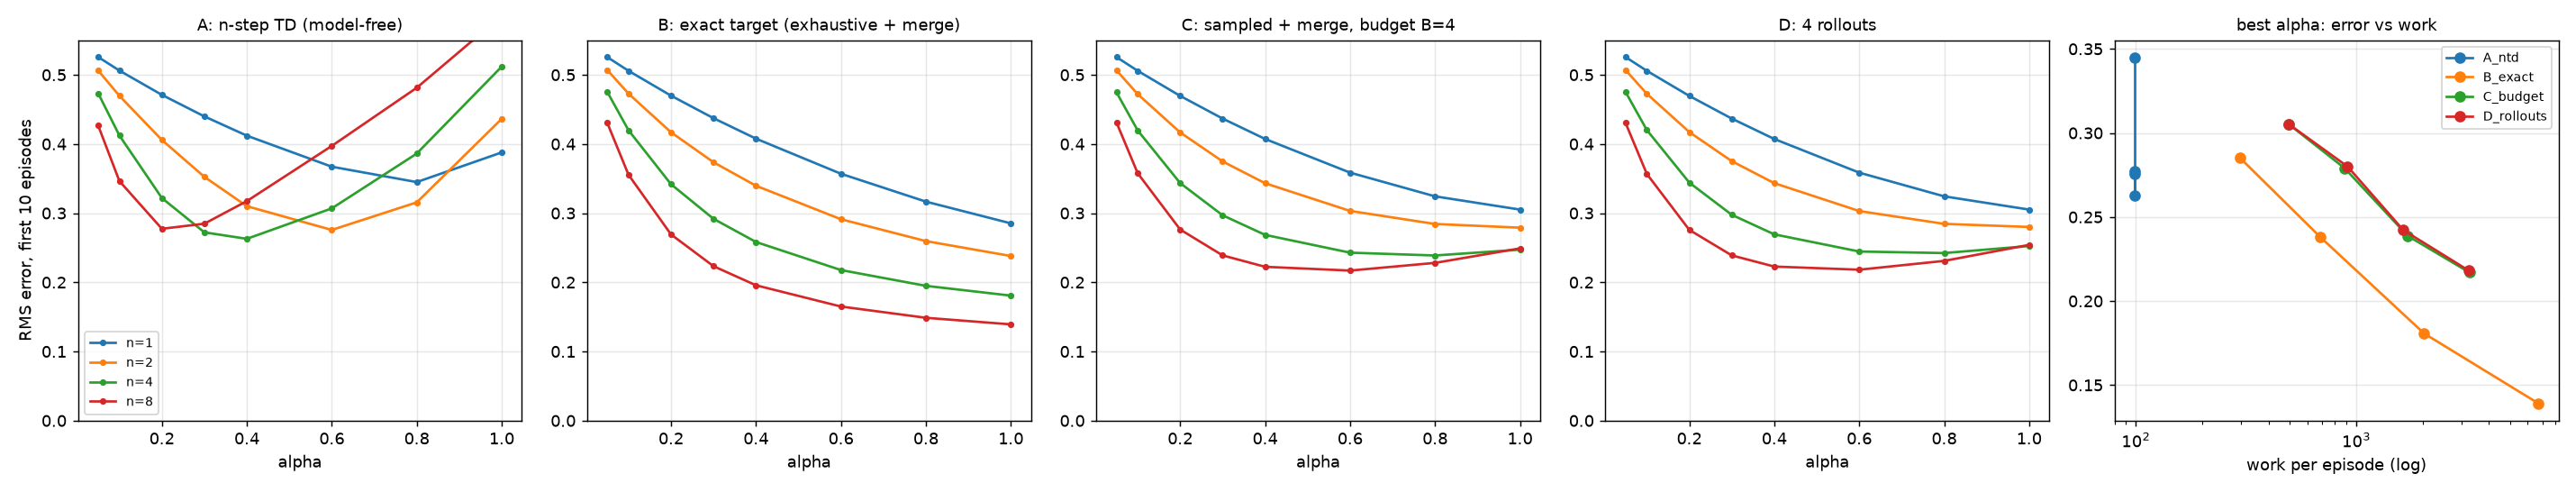
\includegraphics[width=\linewidth]{t1_nstep_td.png}
\caption{T1: 19-state random walk, n-step TD prediction: error against step size for each target, and best-$\alpha$ error against work.}
\end{figure}



\subsection{T2: slippery FrozenLake 8$\times$8, prediction}
\label{sec:t2}
\begin{center}\small
\begin{tabular}{@{}lrrrr@{}}
\toprule
\textbf{Target} & \textbf{n=1} & \textbf{n=2} & \textbf{n=4} & \textbf{n=8}\\
\midrule
A: n-step TD (model-free) & 0.185\,$\pm$\,0.002 & 0.174\,$\pm$\,0.002 & 0.166\,$\pm$\,0.002 & 0.161\,$\pm$\,0.002\\
\quad best $\alpha$, work/episode & $\alpha$=0.6, 42 & $\alpha$=0.4, 42 & $\alpha$=0.4, 42 & $\alpha$=0.2, 42\\[2pt]
B: exact (exhaustive + merge) & 0.159\,$\pm$\,0.002 & 0.137\,$\pm$\,0.002 & 0.114\,$\pm$\,0.003 & 0.094\,$\pm$\,0.003\\
\quad best $\alpha$, work/episode & $\alpha$=1, 205 & $\alpha$=1, 804 & $\alpha$=1, 4{,}067 & $\alpha$=1, 21{,}502\\[2pt]
C: sampled + merge + budget & 0.168\,$\pm$\,0.002 & 0.147\,$\pm$\,0.003 & 0.135\,$\pm$\,0.003 & 0.124\,$\pm$\,0.002\\
\quad best $\alpha$, work/episode & $\alpha$=1, 201 & $\alpha$=1, 380 & $\alpha$=0.8, 676 & $\alpha$=0.6, 1{,}358\\[2pt]
D: independent rollouts & 0.168\,$\pm$\,0.002 & 0.150\,$\pm$\,0.003 & 0.135\,$\pm$\,0.003 & 0.123\,$\pm$\,0.002\\
\quad best $\alpha$, work/episode & $\alpha$=1, 201 & $\alpha$=1, 359 & $\alpha$=0.8, 694 & $\alpha$=0.6, 1{,}227\\[2pt]
\bottomrule
\end{tabular}
\end{center}
\noindent Best step size per cell. RMS error over nonterminal states, averaged over the first 30 episodes and 50 runs (exploring starts; $\varepsilon=0.2$-soft optimal policy; $\gamma=0.99$). Work counts transitions examined or sampled, including the agent's own steps.

\begin{figure}[h]\centering
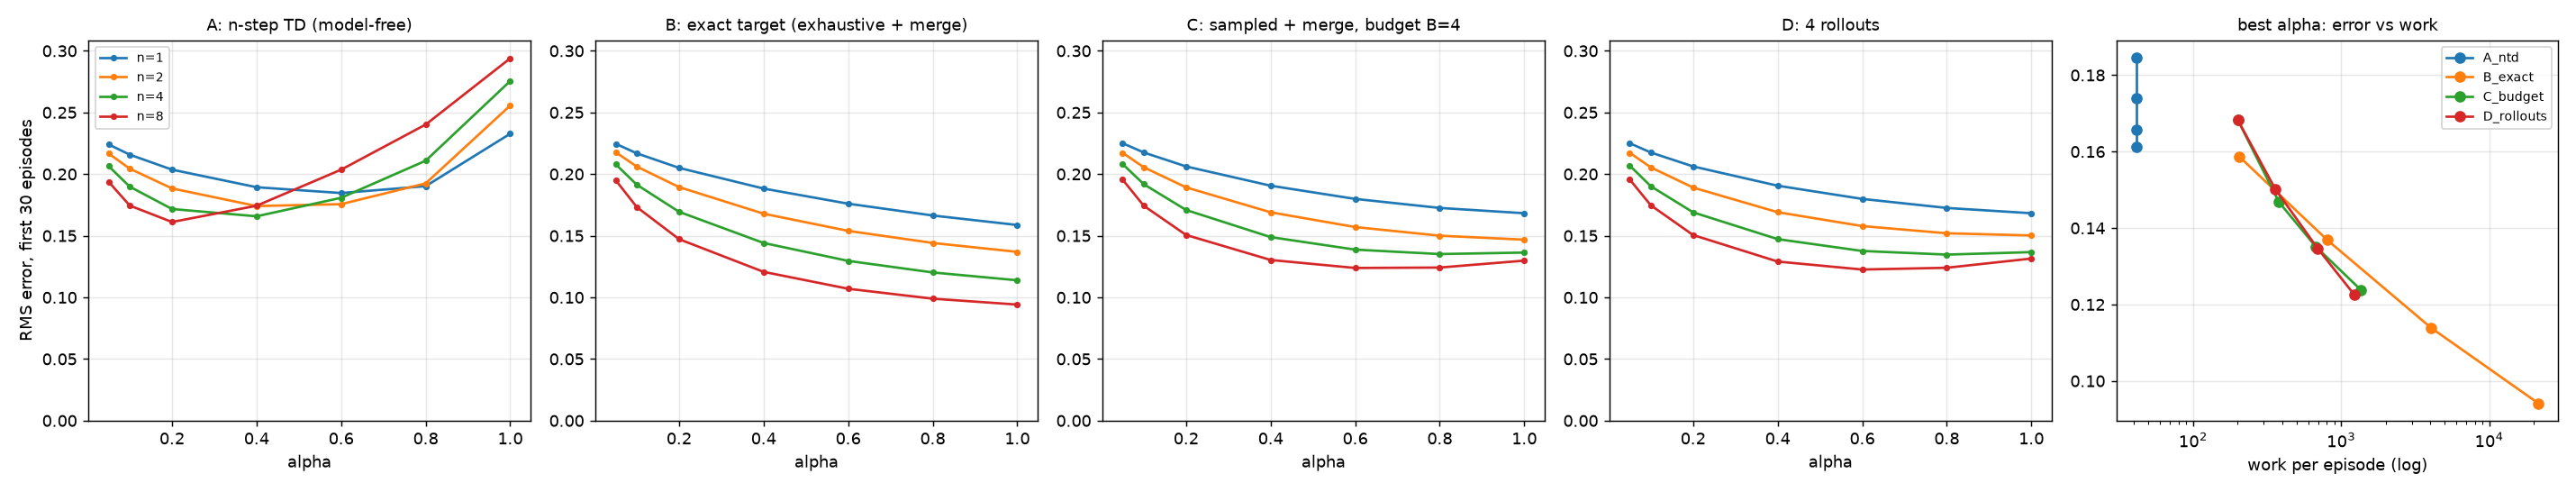
\includegraphics[width=\linewidth]{t2_frozenlake_prediction.png}
\caption{T2: slippery FrozenLake 8$\times$8, prediction: error against step size for each target, and best-$\alpha$ error against work.}
\end{figure}



\subsection{What R1 shows}
\begin{enumerate}
\item \textbf{The baseline is reproduced.} A reproduces Sutton \& Barto's Figure 7.2 on T1: intermediate n is best
  ($n=4$, RMS 0.263 at $\alpha=0.4$), with the characteristic U-shaped curves in $\alpha$.
\item \textbf{Per episode of real experience, the exact target wins clearly.} On T1, B with $n=8$ reaches RMS
  $0.139$ against $0.263$ for the best model-free setting, roughly half the error after the same 10 episodes. On T2 it is
  $0.094$ against $0.161$. B's error falls steadily with $n$ and is best at $\alpha=1$ in every cell: the exact target
  has no sampling noise, so there is no reason to average it.
\item \textbf{Merging with a budget ties with independent rollouts, again.} C and D agree within one standard error in
  every cell of both studies (e.g. T1, $n=8$: $0.217$ vs $0.218$; T2, $n=8$: $0.124$ vs $0.123$). This matches the
  variance study in Section~\ref{sec:variance}: for sampled expected-value targets, merging with reallocation is as
  good as, but not better than, independent sampling.
\item \textbf{Per unit of compute, the picture depends on the problem.} On T1 the exact target dominates the sampled ones
  at equal work (right panel: B's curve lies below C and D everywhere; e.g. $0.181$ at 2{,}030 work vs $0.217$ at about
  3{,}250). On T2 the three are about level at equal work (e.g. B $n=2$: $0.137$ at 804; C/D $n=4$: $0.135$ at about
  690). B buys lower error at higher cost, because an $\varepsilon$-soft policy on slippery ice has up to 12 successors per
  state and the merged frontier quickly covers much of the grid.
\item \textbf{Against model-free TD, the comparison is about which resource is scarce.} B--D spend 3--500$\times$ more work
  per episode than A. If real experience is expensive and a simulator is available (the DEVS setting), the paratemporal
  targets are much better. If compute and experience cost the same, model-free TD with more episodes remains
  competitive on these small problems.
\end{enumerate}

\paragraph{Consequences for the next phases.}
\begin{itemize}
\item The case for exact expansion with merging is strongest when the \emph{reachable merged frontier stays small}:
  work per target is bounded by $n \times |\text{frontier}| \times \text{branching}$, independent of the number of paths,
  while a sampled estimate needs ever more samples for the same accuracy. Next: measure where exact expansion's work
  saturates as $n$ grows, and how many samples C/D need to match B's error.
\item Hybrid selection (exact on small discrete draws, sampled elsewhere) is the configuration to test next. On T2 the
  natural split is to enumerate the slip (3 outcomes) and sample the policy, or the reverse.
\item Control (T2 with n-step Q-learning or SARSA targets) and the Java engine via JPype (R3) are the next steps. The
  Python estimators above are the reference the Java results must match.
\end{itemize}
